\title{Data Mining - Aufgabenblatt 3}
\author{Andra Herta, Tobias Dreher}
\date{08.11.2011}

\documentclass[%
	pdftex,%              PDFTex verwenden da wir ausschliesslich ein PDF erzeugen.
	oneside,%             Einseitiger Druck.
	12pt,%                Grosse Schrift, besser geeignet für A4.
	parskip=half,%        Halbe Zeile Abstand zwischen Absätzen.
	headsepline,%         Linie nach Kopfzeile.
	footsepline,%         Linie vor Fusszeile.
	bibtotocnumbered,%    Literaturverzeichnis im Inhaltsverzeichnis nummeriert einfügen
]{scrartcl}

\usepackage[utf8]{inputenc}
\usepackage[T1]{fontenc}
\usepackage[ngerman]{babel}

\usepackage{amsmath}
\usepackage{amssymb}

\usepackage{libertine}

\usepackage{graphicx}

\usepackage{placeins}
 

\begin{document}
\maketitle

\section*{Aufgabe 7}
\begin{table}[htb]
  \centering
  \begin{tabular}{c|c}
    \textbf{Variable} & \textbf{Einstellung}\\
    \hline
    $t_{max}$ & 12\\
    $k$ & 2\\
    $n_{min}$ & 1\\
  \end{tabular}
\end{table}

\[C = {(1,0),(2,0),(0,1),(2,2),(3,3),(2,3)}\]

\subsection*{$t = 0$}
\[C_{1}(0) = {(2,0),(3,3),(2,2)}\]
\[C_{2}(0) = {(1,0),(0,1),(2,3)}\]

\subsection*{$t = 1$, $x_{\mu} = (1,0)$}
\[D_{var}(C(t)) = 12\]
\[D_{var}(C_{j}(t)) = 12,75\]
\[C_{1}(t) = {(2,0),(3,3),(2,2)}\]
\[C_{2}(t) = {(1,0),(0,1),(2,3)}\]

\subsection*{$t = 2$, $x_{\mu} = (2,0)$}
\[D_{var}(C(t)) = 12\]
\[D_{var}(C_{j}(t)) = 9,75\]
\[C_{1}(t) = {(3,3),(2,2)}\]
\[C_{2}(t) = {(1,0),(0,1),(2,3),(2,0)}\]

\subsection*{$t = 3$, $x_{\mu} = (0,1)$}
\[D_{var}(C(t)) = 9,75\]
\[D_{var}(C_{j}(t)) = 13,33\]
\[C_{1}(t) = {(3,3),(2,2)}\]
\[C_{2}(t) = {(1,0),(0,1),(2,3),(2,0)}\]

\subsection*{$t = 4$, $x_{\mu} = (2,2)$}
\[D_{var}(C(t)) = 9,75\]
\[D_{var}(C_{j}(t)) = 10\]
\[C_{1}(t) = {(3,3),(2,2)}\]
\[C_{2}(t) = {(1,0),(0,1),(2,3),(2,0)}\]

\subsection*{$t = 5$, $x_{\mu} = (3,3)$}
\[D_{var}(C(t)) = 9,75\]
\[D_{var}(C_{j}(t)) = 14,4\]
\[C_{1}(t) = {(3,3),(2,2)}\]
\[C_{2}(t) = {(1,0),(0,1),(2,3),(2,0)}\]

\subsection*{$t = 6$, $x_{\mu} = (2,3)$}
\[D_{var}(C(t)) = 9,75\]
\[D_{var}(C_{j}(t)) = 4\]
\[C_{1}(t) = {(3,3),(2,2),(2,3)}\]
\[C_{2}(t) = {(1,0),(0,1),(2,0)}\]

\subsection*{$t = 7$, $x_{\mu} = (1,0)$}
\[D_{var}(C(t)) = 4\]
\[D_{var}(C_{j}(t)) = 10,5\]
\[C_{1}(t) = {(3,3),(2,2),(2,3)}\]
\[C_{2}(t) = {(1,0),(0,1),(2,0)}\]

\subsection*{$t = 8$, $x_{\mu} = (2,0)$}
\[D_{var}(C(t)) = 4\]
\[D_{var}(C_{j}(t)) = 7,75\]
\[C_{1}(t) = {(3,3),(2,2),(2,3)}\]
\[C_{2}(t) = {(1,0),(0,1),(2,0)}\]

\subsection*{$t = 9$, $x_{\mu} = (0,1)$}
\[D_{var}(C(t)) = 4\]
\[D_{var}(C_{j}(t)) = 8\]
\[C_{1}(t) = {(3,3),(2,2),(2,3)}\]
\[C_{2}(t) = {(1,0),(0,1),(2,0)}\]

\subsection*{$t = 10$, $x_{\mu} = (2,2)$}
\[D_{var}(C(t)) = 4\]
\[D_{var}(C_{j}(t)) = 6\]
\[C_{1}(t) = {(3,3),(2,2),(2,3)}\]
\[C_{2}(t) = {(1,0),(0,1),(2,0)}\]

\subsection*{$t = 11$, $x_{\mu} = (3,3)$}
\[D_{var}(C(t)) = 4\]
\[D_{var}(C_{j}(t)) = 7,5\]
\[C_{1}(t) = {(3,3),(2,2),(2,3)}\]
\[C_{2}(t) = {(1,0),(0,1),(2,0)}\]

\subsection*{$t = 12$, $x_{\mu} = (2,3)$}
\[D_{var}(C(t)) = 4\]
\[D_{var}(C_{j}(t)) = 9,75\]
\[C_{1}(t) = {(3,3),(2,2),(2,3)}\]
\[C_{2}(t) = {(1,0),(0,1),(2,0)}\]



\FloatBarrier
\newpage
\section*{Aufgabe 8}
Da das Austauschverfahren lediglich zu einem lokalen Optimum führt, stellt die Abbildung \ref{fig:aufg8} auch ein solches dar. Jedoch konnte auch nach mehrmaliger Ausführung $D_{var} = 1201$ nie unterschritten werden. 
\begin{table}[htb]
  \centering
  \begin{tabular}{c|c}
    \textbf{Variable} & \textbf{Einstellung}\\
    \hline
    $t_{max}$ & 500\\
    $k$ & 3\\
    $n_{min}$ & 1\\
  \end{tabular}
\end{table}
\begin{figure}[h]
	\centering
	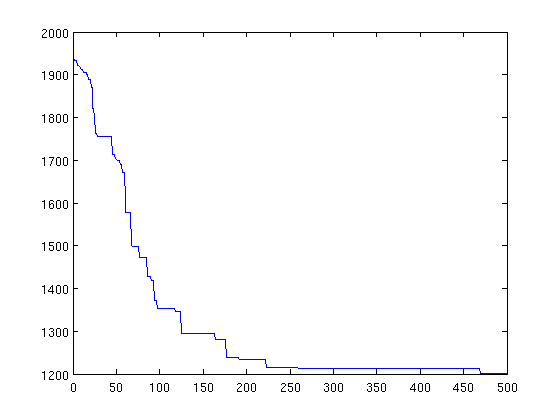
\includegraphics[width=0.8\textwidth]{../80X-Plot.png}
	\caption{Verlauf von $D_{var}$}
	\label{fig:aufg8}
\end{figure}
\end{document}
